%
% File acl2014.tex
%
% Contact: koller@ling.uni-potsdam.de, yusuke@nii.ac.jp
%%
%% Based on the style files for ACL-2013, which were, in turn,
%% Based on the style files for ACL-2012, which were, in turn,
%% based on the style files for ACL-2011, which were, in turn, 
%% based on the style files for ACL-2010, which were, in turn, 
%% based on the style files for ACL-IJCNLP-2009, which were, in turn,
%% based on the style files for EACL-2009 and IJCNLP-2008...

%% Based on the style files for EACL 2006 by 
%%e.agirre@ehu.es or Sergi.Balari@uab.es
%% and that of ACL 08 by Joakim Nivre and Noah Smith

\documentclass[11pt]{article}
\usepackage{acl2014}
\usepackage{times}
\usepackage{url}
\usepackage{latexsym}
\usepackage{tabulary}
\usepackage{tabulary}
\usepackage{comment}
\usepackage{graphicx}
%\setlength\titlebox{5cm}

% You can expand the titlebox if you need extra space
% to show all the authors. Please do not make the titlebox
% smaller than 5cm (the original size); we will check this
% in the camera-ready version and ask you to change it back.

\title{Toward Macro-Insights  for Suicide Prevention: \\ Anaylzing Fine-Grain Distress at Scale}

%\author{Ravdeep Johar\\
 % Department of Computer Science \\
 % Rochester Institute of Technology \\
 % {\tt rsj7209@rit.edu} \And
 %Christopher M. Homan\\
 % Department of Computer Science \\
 % Rochester Institute of Technology \\
  %{\tt cmh@cs.rit.edu}\\\\ 
 %}

\date{March 21, 2014}

\begin{document}
\maketitle
\begin{abstract}

This paper is an initial exploratory research 
 \end{abstract}

\section{Introduction}


Suicide is among the top ten---top five for indiviuals 10--44 years in age---leading causes of death in the United States \cite{heron2009deaths}. Indeed, while mortality rates for most illnesses decreased between 2008 and 2009, the rate of suicide increased by 2.4\%  \cite{heron2009deaths}. The lifetime prevalence for suicidal ideation is between 5.6 and 14.3 percent, with an even greater prevalence among youth (19.8–24.0\%) \cite{nock2008suicide}. 

Individuals may be more inclined to seek support from informal resources such as social media networks instead of seeking treatment (Crosby et al., 2011; Bruffaerts et al., 2011; Ryan et al., 2010). Evidence suggests that youth and emerging adults usually prefer to seek help from their friends and families; however, higher levels of suicidal ideation are associated with lower levels of help-seeking from both formal or informal resources (Deane et al., 2001).  Identifying risk factors associated with suicide is the first step towards prevention, and ideally someone with expertise would do this.  Due to social stigma among other barriers, individuals with suicidal ideation may not always reach out to professionals. However, trends in help-seeking suggests that social media might be a rich outlet for learning about support seeking.

It would seem, then, that any significant improvement of clinical preventative measures could also be bolstered by utilizing non-expert or automated detection. 
Internet- and telecommunications-driven activity is revolutionizing the social sciences by providing data---much of it publicly available---on human activity in situ, at volumes and a level of time and space granularity never before approached. Can such data improve clinical preventative measures by providing access to at-risk individuals who would otherwise go undected, and by leading to better science about suicide risk behaviors? This question is the focus of our study.


To test this question, we use linguistic modeling to classify, at the level of individual tweets, risk factors for suicidal  behavior from a highly-connected, geographically dense collection of twitter users. We then use the scale of our data to aggregate the classification, which at the tweet level is very noisy, into a method for detecting highly at-risk individuals. Our classification scheme involves training by both experts and non-experts, and outperforms very reasonable and baseline approaches.

\begin{comment}
\textbf{[CMH: Vince or Megan, please elaborate. I'm looking for terse, citable facts about suicide]} Suicide is epidemic in some populations. It is the th leading cause of death. In nearly all populations, it is on the rise.

\textbf{[CMH: Vince or Megan, I'm making a lot of claims about clinical practice complete ad hoc. Please rewrite as necessary.]} From a clinical perspective, suicide is a social-behavioral problem one that is related to other social-behavioral problems, such as depression or drug addiction. Unfortunately, due to a number of reasons, including social stigma, individuals afflicted with such pre-suicidal conditions can often not be replied upon to report their behavior.  Suicidal behavior is usually not discovered until the victim acts, and even then diagnosis is muddy. 

Suicide is extremely infrequent and usually the result of psychological distress that takes several weeks at the very least to manifest. How can social media and its primary virtues, namely high sample rates and volume [maybe a reference here to that Alex Pentland diagram, Vince?], help to detect suicidality? Certainly, one would expect that within the sheer volume of data that the most popular social media services produce must lie some evidence of suicide ideation. Suicidal behavior, however, is extremely difficult to diagnose even in the best of situations. Rather than pick out obvious rare cases, our goal here is to detect in the language of microblog users expressions 
of behavior or ideas related to suicide. Most of this language will, of course, not indicate actual suicide ideation... [something about painting a picture of how factors related to suicide lie in a virtual social space.]

In contrast to the way that suicide is detecting in clinical settings [Megan, hopefully you will say something about this in the clinical subsection above], the high sample rates that social media provide allow us to detect clues of suicide-related behavior as they occur, without relying on self reporting by often highly unreliable sources. 


\subsection{Research Questions}
\begin{description}
\item[R1] Using support vector machines trained on primarily linguistic features, can we learn to classify tweets as whether or not they express ideas related to suicide?
\item[R2] Can network structure enhance such classification models?
\item[R3] Can we predict the expression of suicide-related ideas in the future?
\end{description}
\end{comment}

\section{Related Work}
\subsection{Clinical}
Based on what we already know, it is reasonable to expect that a better understanding of risk factors for suicidal behaviors (i.e., suicidal ideation and suicide attempt) will lead to more effective clinical practices. Approximately one third of individuals who reported lifetime suicidal ideation made a plan and nearly three-quarters of those who reported having a suicide plan went on to attempt suicide \cite{kessler1999prevalence}. According to Kessler, Borges, and Walters  \cite{kessler1999prevalence}, the odds of attempting suicide increased exponentially when individuals endorsed three of more risk factors (e.g., having a mood or substance abused disorder). Might traces of suicide plans and other risk factors leave detectable, meaningful traces in social media?

Data on suicide is traditionally oftern collected primarily from healthcare organizations or large scale studies that are often limited depending on providers' ability to assess and document suicide risk, or from self-report measures \cite{crosby2011self,horowitz2009suicide}.  Traditional methods for researching suicidal behavior is influenced by sociocultural barriers such as stigma and shame, as well as issues with methodology \cite{crosby2011self}. For these reasons, and because of the fundamentally subjective nature of the problem, data on suicide is never particularly reliable. 

	Aside from demographic variables, previous suicide attempts, mental health concerns (i.e., depression, substance abuse, suicidal ideation, self-harm, and impulsivity), family history of suicide, interpersonal conflicts (i.e., family violence and bullying), mechanism or means for suicidal behavior (e.g., firearms)  are commonly cited risk factors for suicidal behavior \cite{nock2008suicide,crosby2011self,gaynes2004screening,harriss2005suicidal,shaffer2004columbia,shaffer2004columbia,brown2000risk}. 

Suicide is a complex phenomenon with a low base rate; therefore, many researchers tend to focus on examining the relationship between risk factors and suicidal behavior without relying heavily on theoretical models \cite{nock2008suicide} . However, Mann, Waternaux, Haas, and Malone (1999), developed the stress diathesis model for suicidal behavior using many of the aforementioned risk factors.  Specifically, this framework suggests that objective states such as(e.g.,  depression and life events) as well as subjective states and traits such as a (e.g., family history of depression and/or suicide as well as substance abuse) were among the risk factors that contributed to suicidal ideation and could eventually lead to either externalizing (e.g., interpersonal violence) or internalizing aggression (e.g., attempting suicide) (Mann et al., 1999).

	Since the stress-diathesis model was developed using risk factors for suicidal behavior, it is the ideal framework to analyze publically available linguistic data from social media outlets such as Twitter. While traditional methods are limited by survey questions or clinical reports, data from social media can be used as a natural experiment to examine depression and suicidal ideation without being constrained by such sample biases as individuals who are willing take part in research and/or seek out formal sources of support. Moreover, this natural experiment method may provide information about individuals who are unlikely to engage in formal help-seeking behaviors and eventually it could be used to identify effective methods in natural helping. Hence, this universal approach to screening for suicidal behaviors may have future implications not only for identifying individuals who have a higher prevalence for suicidal behaviors but it could eventually lead to the methods for enhancing protective factors against suicide.  


\subsection{Affect Detection and Clinical Expertise}
\subsection{Affect in Social Media}

Sentiment analysis has been widely studied in a number of computational settings, including on various social networking sites. Relatively little of this work has focused on suicide or related psychological conditions. \cite{masuda2013suicide} study suicide on mixi. \cite{cheng2012opportunities} consider the ethical and political implications of online data collection for suicide prevention. \cite{Jay} show correlations between frequency in tweets related to suicide and actual suicide in the 50 United States of America. \cite{sadilek2014modeling} study depression on Twitter. De Choudhury and collaborators studied depression---in general and post-partem---in Twitter~\cite{de2012not,de2012happy,de2013major,de2013understanding} and Facebook~\cite{de2014characterizing}. Homan et al. investigate depression in TrevorSpace~\cite{homan2014social}. A number of social theories of suicide have been proposed~\cite{wray2011sociology}. Most of this work was with respect to offline social systems. 

A rather substantial body of work already exists on the use of Twitter to study emotion~\cite{bollen2011twitter,dodds2011temporal,wang2012harnessing,pfitzner2012emotional,kim2012you,bollen2011happiness,pfitzner2012emotional,bollen2011modeling,mohammad2012emotional,golder2011diurnal,de2012not,de2012happy,de2013major,de2013understanding,hannak2012tweetin,thelwall2011sentiment,pak2010twitter}. For instance,
Golder and and Macy study aggregate global trends in ``mood,'' and show, for example, that people wake up in a relatively good mood that decays as the day progresses \cite{golder2011diurnal}, Bollen et al.~\cite{bollen2011modeling} show that POMS-scored tweets are often tied to current events, such as elections and holidays.

A common theme in social network analysis is that actors who share ties generally share similar properties. A widely-used~\cite{bliss2012twitter,coviello2014,bollen2011happiness} metric for testing the overall similarity between 
actors in a network for some property $X$ is \emph{assortativity}, defined as  the Pearson correlation coefficient~\cite{newman2002assortative} of $X$ over all pairs of actors who share a tie.  One line of research seeks
to discover the mechanism through which such correlations occur~\cite{newman2002assortative}. 
At the most fundamental level, this is a matter of whether like individuals seek each other out (called selection, or---confusingly enough---homophily) or whether related individuals influence one another. Teasing apart which of these two processes can be rather challenging and generally requires some level of experimental design~\cite{centola2010spread,centola2011experimental}
For instance, Coviello et al. study the spread of mood in Twitter~\cite{coviello2014}. They notice a very small---but statistically significant---spreading of mood over Facebook. 

From the clinical perspective of detecting individuals who exhibit a high risk for committing suicide, determining  causality remains a challenge to this multidimensional problem; however, finding patterns in the social interactions of individuals who commit suicide may provide additional insight. For our purposes, then a more relevant theory is perhaps that of social support~\cite{wellman1990different} which seeks to clarify the social forces---protective, preventative, persuasive, or coercive---that affect behavior. 

At the most basic level, one can distinguish between \emph{weak} and \emph{strong} social ties and observe different behavior and effects between them.  

Following in the work of Bliss et al.~\cite{coviello2014} and Bollen et al.~\cite{bollen2011happiness} we show that 
mood is assortative. We additionally consider the predictive power of various measureable notions of tie strength.
We study suicide risk factors here but we would expect our methods would apply to other domains.



\section{Methods}
\subsection{Overview}
\textbf{CMH: Mention coding as the method of obtaining ground truth; provide justification for it.}
\subsection{Data}
Twitter is a worldwide popular social networking and microblogging service. Twitter message contains up to 140 words each and such words limit encourages users to update frequently. User's regular posts on Twitter have been used to predict depression[Munmun De Choudhury et al., 2013], influenza-like illnesses[Adam Sadilek et al., 2012] in previous studies. Our research looked into an old Twitter dataset originated from the New York City, which covered a month long period since May 18, 2010, total with about 2.5 million tweets from 6,237 unique users. See Table~\ref{table::dataset}.

\begin{table}[t]
\small
\centering
\begin{tabular}{ l | r }
\multicolumn{2}{c}{\textbf{New York City Dataset}} \\
\hline
\textbf{Unique users}&       632,611      \\
\hline
\textbf{Unique geo-active users}&        6,237       \\
\hline
\textbf{Tweets total}&        15,944,084\\
\hline
\textbf{GPS-tagged tweets}&   4,405,961\\
\hline
\textbf{GPS-tagged tweets by geo-active users}&  2,535,706\\
\hline
\textbf{GPS-tagged tweets by geo-active users}&  2,047 \\
\textbf{that show a symptom of an illness}&\\
\hline
\textbf{``Follows'' relationships}&  102,739  \\
\textbf{between geo-active users}&\\
\hline
\textbf{``Friends'' relationships}&   31,874   \\
\textbf{between geo-active users}&\\
\end{tabular}
\caption{\small Summary statistics of the data collected from NYC. Geo-active users are people who geo-tag their tweets relatively frequently (more than 100 times per month). Note that the reciprocity rate in the social graph is about 31\%, which is consistent with previous findings  cite what is twitter.} 
\label{table::dataset}
\end{table}
\subsection{Data Collection}
-slang replace
-strip punctuations

\textbf{CMH: \cite{Jay}. It is important to give them credit for what they did, and to note that the scheme you describe was adopted from them almost verbatim.}

To identify suspected suicide tweets, we created a list of inclusive search terms/phrases according to various risk factors and warning signs linked to suicide. [Table 1]



Among these, terms in Sad category were generated from LIWC [http://www.liwc.net/index.php]. All the rest were concluded from depression and other psychological disorders (Lewinsohn, Rohde, \& Seely, 1994), prior suicide attempts (Lewinsohn et al., 1994), family violence, family history of drug abuse, firearms in the home, and exposure to the suicidal behavior of others (National Insti- tute of Mental Health, 2012). Other search terms included common antidepressants, as well as phrases that indicated suicide (Hawton, Zahl, \& Weaterall, 2003), ideation (American Foundation for Suicide Prevention, 2012a), deliberate self-harm (Zahl \& Hawton, 2004), bullying (Klomek, Sourander, \& Gould, 2011), feelings of isolation (CDC, 2012), and impulsiveness (American Foundation for Suicide Prevention, 2012b). [Self-directed Violence Surveillance: Uniform Definitions and Recommended Data Elements, report from Megan]

Before searching, we did some kinds of preprocess work:  (1) converted all text to lower case (2) stripped out all the punctuations and special characters; (3) built a slang dictionary which contains 5424 text slang based on online resources [http://www.noslang.com/dictionary/], Internet slang, and abbreviations. We replaced all the matching items fount in the dataset with corresponding easy read words. These two steps helped us extract more suicide-related tweets for analysis in the following process.


\subsection{Preprocess}
-stopwords
-keep stemming words

Using Scikit-learn package(http://scikit-learn.org/stable/about.html\#citing-scikit-learn), it is very simple to remove stop words (like ``and'', ``the'', etc.) with parameter ``stop\_words'' tuned as ``string \{`english'\}''. 

At the same time, we kept original words without any word stemming, i.e.: ``computers'', ``computing'', and ``compute'', neither of these words will be mapped to the same stem ``comput''. The reason here is: a tweet containing like ``soooooooooo sad!" is supposed to convey stronger emotions than simple ``so sad''.

\subsection{Ground Truth}
The dataset is divided into two equal parts, each set is annotated by two experts. The first dataset is annotated by experts in Computing Science and Linguistics  the other set by clinical experts in Psychology. Each dataset was annotated by male and female pairs. The reasoning behind this method is to analyze the difference of perceptions between male and female, and, also between experts VS non-experts in psychology.

\begin{figure}
\centering
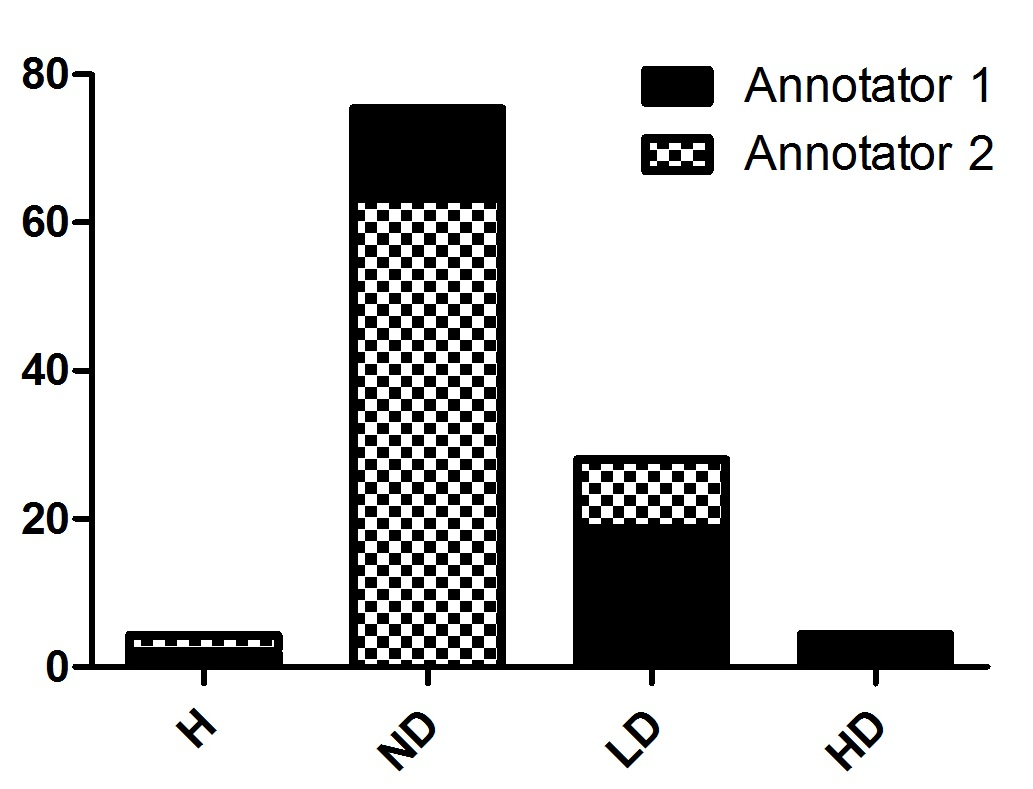
\includegraphics[scale=0.7]{ChrisCissi4cat.jpg}
\end{figure}

\begin{figure}
\centering
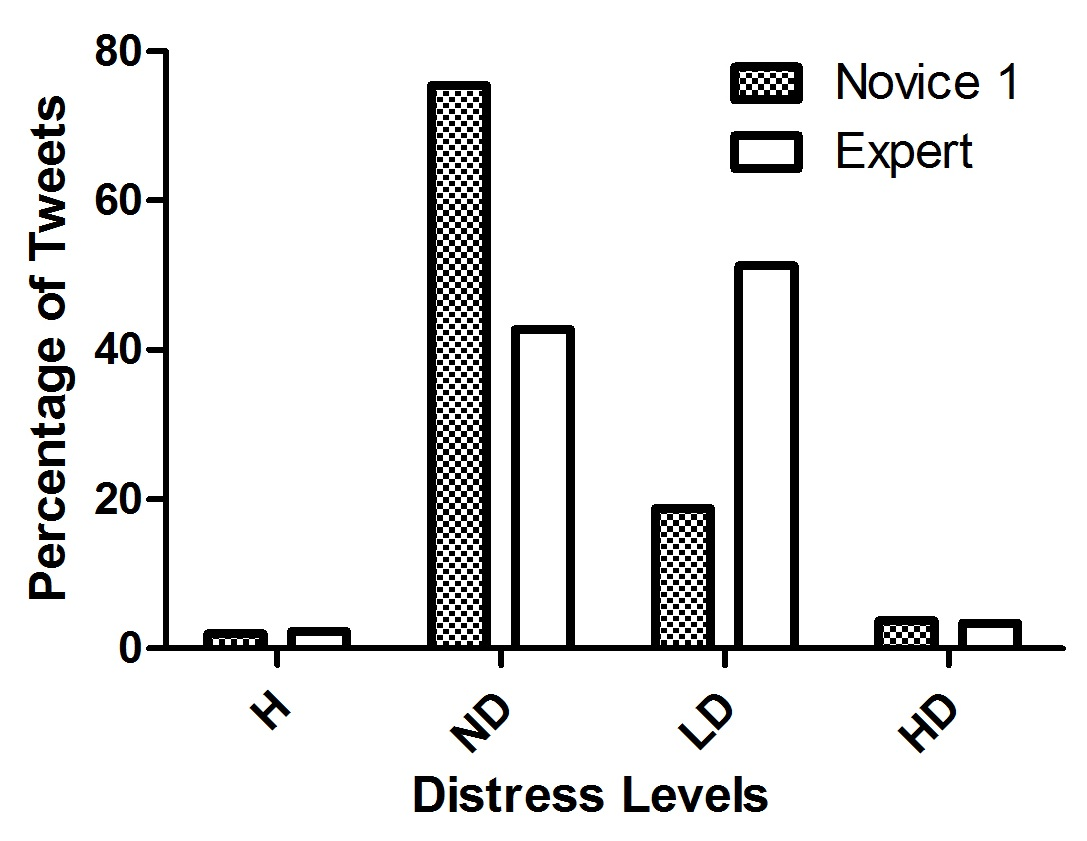
\includegraphics[scale=0.7]{ChrisMegan4Cat.jpg}
\end{figure}

For annotation process each tweet was provided with a context, i.e. three tweets before and after the tweet to be annotated, along with timestamp of these tweets and thematic category to which the tweet belonged to. Each tweet was annotated for distress level and thematic category. The distress level was divided into four categories: High Distress(HD), Low Distress(LD), No Distress(ND) and Happy(H), whereas, for the thematic category the annotaters labeled just yes or no based on whether the thematic category applied to the tweet or not.

\begin{table}
    \centering
    \begin{tabular}{|l|l|l|l|l|}
    \hline
    Annotator    & H   & ND   & LD   & HD  \\ \hline
    Annotator 1  & 2.0 & 75.4 & 18.8 & 3.8 \\ \hline
    Annotator 2  & 4.3 & 63.3 & 28.0 & 4.4 \\ \hline
    Annotator 3  & 2.3 & 42.8 & 51.3 & 3.4 \\ \hline
    Annotator 4  & ~   & ~    & ~    & ~   \\ \hline
    \end{tabular}
    \caption {percentage of distress labels }

\label{tab:percentage}
\end{table}


\subsection{Topic Modeling}

Toping modeling is often used to analyze text data by finding topics within a corpus of documents. Each topic consists of words that occur together frequently. These models are capable of connecting words with similar meanings and distinguish words with multiple meanings. We utilize  Latent Dirichlet Algorithm  \cite{Blei} to create these topics, in this method the documents (in our case tweets) are represented as random mixtures over latent topic where each topic is characterized by a distribution over words (REPHRASE). 

We perform topic modeling on our dataset to compare the topics within high distress and everyday tweets. Before performing the topic modeling, the stop words and words that occur only once in the dataset are removed. The LDA algorithm is then applied to create $5$ topics using $100$ iterations, Table \ref{tab:tm} shows the results.

\begin{table}[h]
    \centering
    \begin{tabular}{|p{0.7cm}|p{4cm}|}
    \hline
    \textbf{Topic No } & \textbf{Words} \\ \hline
    \vfill \vfill Topic 1 & miss u, leave alone, sleep forever, win lose, gon lose, left alone, \#iconfess hate, lost best, best friend, think insomnia \\ \hline
    \vfill \vfill Topic 2 & hate job, feel sad, don't wanna, feel helpless, bed lonely, feel better, miss you, sad =/, tired everything, miss love\\ \hline
    \vfill \vfill Topic 3 & miss you!, wanna cry, committing suicide, tired living, miss 2, one person, broke bitches, worst feeling, leave world, bout go \\ \hline
    \vfill \vfill Topic 4 & commit suicide, get hurt, miss baby, feel empty, :( miss, lost phone, don't let, drug overdose, can't wait, \@ work \\ \hline
     \vfill \vfill Topic 5 & feel like, tummy hurts, lost friend, ima miss, deserve die, right now..., hurts :(, get fat, every day, like crying  \\ \hline
    \end{tabular}
 \caption {Topic Analysis on bigrams of High Distress Tweets }

\label{tab:tm}
\end{table}

\subsection{Analysis}
-topic modeling \cite{Blei}

\subsection{features}

To prepare the tweets for the classifier, we extract features using the unigram, bigram and trigram model. For example, a simple tweet ``I am so happy'' is represented as the following feature vector: \{I, am, so, happy, I am, am so, so happy, I am so, am so happy\}. The tf-idf values were calculated for each attribute: tf-idf stands for ``term frequency - inverse document frequency'', which is a numerical statistic to reflect how important a tokenization is to a document in a collection or corpus. The tf-idf value increases proportionally to the number of times a tokenization appears in the dataset, but is offset by the frequency of the tokenization in the corpus, which helps to control for the fact that some words are generally more common than others. With the help of Scikit-learn package(http://scikit-learn.org/stable/about.html\#citing-scikit-learn), there values can be easily acquired. 

\subsection{feature selection}
chi2 feature selection

\subsection{Challenges with Annotation}

There are unique challenges in annotating data from Twitter.  Aside from having to become familiar with different types of slang and abbreviations that could have multiple meanings, this format provides limited background context to inform the annotation process.  Outside of the theoretical informed annotation process, there were emerging themes of aggression, privilege and oppression, and daily struggles, among other.  As a result of the aggressive context, personal bias may have impacted annotation decisions. For instance, numerous tweets contained sarcasm and dark humor which may result in annotators underestimating or overlooking actual distress. In addition, by pulling data from Twitter, critical information such as pictures and the context behind information that has been retweeted.  Specifically, a few individuals retweeted in a humorous manner about what to say to someone who considering suicide; however, without any knowing the circumstances of the original message it was difficult to classify this tweet.  It could represent dark humor or it could be a form of bullying.

\subsection{SVM part}
-scikit learn sth....

\subsection{Network Features}
One of the fundamental properties of social networks appears to be \emph{tie strength}, or how ``close'' socially two people are. A large body of literature suggests that people are more likely to share personal information with stronger ties, and that weak ties play an important role in providing new information.  
Measuring tie strength is problematic, as there is no gold standard here. Social networking services seem to exacerbate the disparity between strong and weak ties, as many have ``friends'' or ``followers'' whom they may not even know personally, and also create their own problems and opportunities for estimating tie strength. In large-scale network analysis, researchers have sometimes characterized tie strength by the 
\emph{embeddedness} of an edge, which is the number of friends in common that two actors sharing a tie have. Highly embedded links are part of a strong social fabric, and represent strong ties. Another method of estimating tie strength is to measure the amount of activity between users. In this study, we investigate both the role that embeddness and activity play in corrolating suicide-related language. 

\section{Results}
\subsection{Strength of Ties}
Table~\ref{tab:strength} shows how the use of sad language (measure by the LIWC sad feature) correlates among users sharing different tie strength and between personal and broadcast messages.

\begin{table}
  \centering
  \begin{tabular}{l|r|r}
Embeddedness    &Broadcast&Personal\\
\hline
0 & 0.046 & 0.098\\
\hline
1 & 0.061 & 0.13\\
\hline
5& 0.082 & 0.23
  \end{tabular}
\label{tab:strength}
\caption{Pearson correlation coefficient of LIWC sad (aggegrated over all tweets collected) of broadcast and reciprocated personal tweets.}
\end{table}
\section{Discussion}

As previously mentioned, many of the risk factors for suicidal behavior may be linked to other expressions of distress such as aggression and interpersonal violence (Mann et al., 1999).  The goal of this study is to classify whether tweets were related to distress or not in order to determine the feasibility of classifying suicidal behaviors.  However, due to the overlap between internal and external expressions of anger, it is difficult to classify suicidal behavior without more contextual information.  Consistent with the stress diathesis model for suicidal behavior, aggression was an emerging theme that arose from the data. A number of individuals tweeted about feeling empty, hopeless, angry, frustrated, and alone.  While these are risk factors for internalizing aggression (i.e., suicidal behavior); these states are also associated with externalizing aggression.  In addition to overt expressions of anger and violence, many of the humorous tweets had an aggressive undertone.  Individuals often exert dominance by using pejorative and derogatory language, and the content of these tweets was often suggestive of past or current distress.  


\subsection{Limitations}
As ground truth, we rely on tweets hand-annotated by experts and non-experts. However, the mental state of another individual, observed from a line or two of text  often written in an informal register is necessarily hard to discern and, even under less noisy conditions, extremely subjective; even the observers' personal understandings of such concepts as ``distress'' may differ drastically. This makes inter-annotator agreement quite a challenge, to say nothing of observation in some objective fashion of the true mental state.


Higher levels of suicidal ideation have an inverse relationship with all types of help-seeking and a positive correlation with the decision to not seek support \cite{deane2001suicidal}. Thus we would expect suicidal individuals to generally be less active on social media than those who are not. (One ray of sunshine is that a number of studies have shown a positive correlation between online social network use and negative mood. Perhaps this means in part that individuals who are depressed are slower to disengage on- rather than off-line.)
 Part of the problem in assessing the effectiveness of self-reporting is the relative rareness by which suicide occurs, and by the inherent subjectivity of the act, which makes any data on suicide fuzzy.
 
\section{Conclusion and Future Work}
\section*{Acknowledgments}


% include your own bib file like this:

\bibliographystyle{acl}
\bibliography{acl2014}

\begin{table*}
    \centering
    \begin{tabulary}{500pt}{|C|C|}
    \hline
    \textbf{Suicide Risk Factor Category} & \textbf{Search Terms and Phrases} \\ \hline
    Depressive Feelings & ~  me abused depressed, tired of living,so depressed,leave this world, wanna die,me hurt depressed, feel hopeless depressed, feel alone depressed, i feel helpless, i feel worthless, i feel sad, i feel empty, i feel anxious, hate my job, feeling guilty, deserve to die, desire to end own life, feeling ignored, tired of everything, feeling blue, have blues                                                                                                                                                                                                                                                                                                                                                                                                                                                                         \\ \hline
    Depression Symptoms                   & sleeping pill, sleeping a lot, i feel irritable, i feel restless, have insomnia, sleep forever,sleep disorder                                                                                                                                                                                                                                                                                                                                                                                                                                                                                                                                                                                                                                                                                                                             \\ \hline
   Drug Abuse                            & depressed alcohol, sertraline, zoloft, prozac, pills depressed, clonazepam, drug overdose, imipramine                                                                                                                                                                                                                                                                                                                                                                                                                                                                                                                                                                                                                                                                                                                                     \\ \hline
  Prior Suicide Attempts                & suicide once more, me abused suicide, pain suicide, tried suicide                                                                                                                                                                                                                                                                                                                                                                                                                                                                                                                                                                                                                                                                                                                                                                         \\ \hline
  Suicide Around Individual             & mom suicide tried, sister suicide tried, brother suicide tried, friend suicide, suicide attempted, suicide attempt                                                                                                                                                                                                                                                                                                                                                                                                                                                                                                                                                                                                                                                                                                                        \\ \hline
   Suicide Ideation                      & commit suicide,committing suicide,feeling suicidal, suicide thought about, thoughts suicide, think suicide, thought killing myself, used thought suicide, once thought suicide, past thought suicide, multiple thought suicide, want to suicide, shoot myself, a gun to head, hang myself, intention to die                                                                                                                                                                                                                                                                                                                                                                                                                                                                                                                               \\ \hline
   Self Harm                             & stop cutting myself, hurt myself, cut myself                                                                                                                                                                                                                                                                                                                                                                                                                                                                                                                                                                                                                                                                                                                                                                                              \\ \hline
   Bullying                              & i am being bullied, i have been cyber bullied, was bullied, feel bullied, stop bullying me, keeps bullying me, always getting bullied                                                                                                                                                                                                                                                                                                                                                                                                                                                                                                                                                                                                                                                                                                     \\ \hline
   Gun Ownership                         & gun suicide, shooting range went, gun range my                                                                                                                                                                                                                                                                                                                                                                                                                                                                                                                                                                                                                                                                                                                                                                                            \\ \hline
   Psychological Disorders               & diagnosed schizophrenia, diagnosed anorexia, diagnosed bulimia, i diagnosed ocd, i diagnosed bipolar, i diagnosed ptsd, diagnosed borderline personality disorder, diagnosed panic disorder, diagnosed social anxiety disorder, diagnosed post traumatic stress disorder, sleep apnea                                                                                                                                                                                                                                                                                                                                                                                                                                                                                                                                                     \\ \hline
   Family Violence Discord               & dad fight again, parents fight again, lost my friend, argument with wife, argument with husband, shouted at each other                                                                                                                                                                                                                                                                                                                                                                                                                                                                                                                                                                                                                                                                                                                    \\ \hline
   Impulsivity                           & i impulsive, i am impulsive                                                                                                                                                                                                                                                                                                                                                                                                                                                                                                                                                                                                                                                                                                                                                                                                               \\ \hline
   Sad                                   & abandon, ache, aching, agoniz, agony, alone, broke,cried, cries, crushed, cry, crying, damag, defeat, depress, depriv, despair, devastat, disadvantage, disappoint, discourag, dishearten, disillusion, dissatisf, doom, dull, empt, fail, fatigu, flunk, gloom, grave, grief, griev, grim, heartbreak, heartbroke, helpless, homesick, hopeless, hurt, inadequa, inferior, isolat, lame, lone, longing, lose, loser, loses, losing, loss, lostlow, melanchol, miser, miss, missed, misses, missing, mourn, neglectoverwhelm, pathetic, pessimis, piti, pity , regret, reject, remorse, resign, ruin, sad, sadde, sadly, sadness, sob, sobbed, sobbing, sobs, solemn, sorrow, suffer, suffered, sufferer, suffering, tears, traged, tragic , unhapp,unimportant, unsuccessful, useless, weep, wept, whine, whining, woe, worthless, yearn \\ \hline

  
    \end{tabulary}
\caption{Search phrases for categories}
  \label{Table:1}
\end{table*}
%  remember to run:
% latex bibtex latex latex
% to resolve all references

\end{document}
